\subsection{UC11- Visualizzazione informazioni sul software}
\begin{figure}[H]
    \centering
    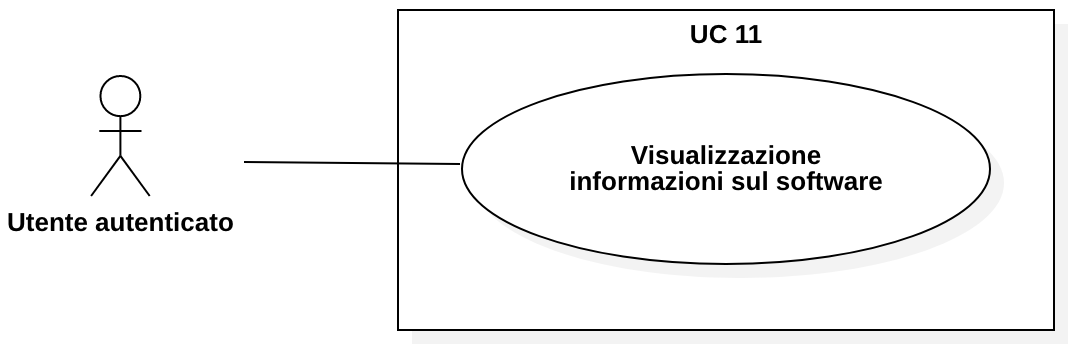
\includegraphics[scale = 0.7]{components/img/UC11.png}
    \caption{UC11 - Visualizzazione informazioni sul software}
\end{figure}
\begin{itemize}
\item \textbf{Attore Primario:} Utente autenticato;
\item \textbf{Precondizione:} Il sistema si trova nella schermata delle impostazioni;
\item \textbf{Postcondizione:} Viene visualizzata una finestra con le informazioni sul software;
\item \textbf{Scenario principale:}
    \begin{enumerate}
    \item L'utente vuole avere informazioni sul software e clicca sull'apposito pulsante;
    \item Il sistema visualizza una finestra apposita con ciò che l'utente ha chiesto.
    \end{enumerate}
\end{itemize}